\documentclass[11pt,a4paper]{article}

\usepackage[margin=0.8in]{geometry}
\usepackage{hyperref}
\usepackage{enumitem}
\usepackage{graphicx}
\usepackage{xcolor}
\usepackage{tikz}
\usepackage{float}

\usetikzlibrary{arrows.meta,positioning,shapes.geometric}

\setlength{\parindent}{0pt}
\setlength{\parskip}{5pt}

\hypersetup{
    colorlinks=true,
    linkcolor=black,
    urlcolor=blue
}

\begin{document}

\begin{center}

{\Large\bfseries
CivicSight: Smart Road Damage Detection\\
and Municipal Repair Management System
}

\vspace{0.4cm}

{\large
\textbf{Project Proposal for UCS503}
}

\vspace{0.15cm}

Submitted to:

\vspace{0.05cm}

\textbf{Ms. Paramveer Kaur}

\vspace{0.05cm}

\textbf{Thapar Institute of Engineering and Technology}

\vspace{0.45cm}


\begin{tabular}{ccc}

\begin{minipage}{0.29\textwidth}
\centering
\textbf{Laksh Garg}\\
Roll No.: \texttt{1024030156}\\
\texttt{lgarg\_be24@thapar.edu}
\end{minipage}

&
\begin{minipage}{0.29\textwidth}
\centering
\textbf{Pranay Mittal}\\
Roll No.: \texttt{1024030159}\\
\texttt{pmittal\_be24@thapar.edu}
\end{minipage}

&
\begin{minipage}{0.29\textwidth}
\centering
\textbf{Devansh Thapar}\\
Roll No.: \texttt{1024030154}\\
\texttt{dthapar\_be24@thapar.edu}
\end{minipage}

\end{tabular}

\end{center}

\vspace{0.25cm}

\section{Higher-order goal}

The goal of CivicSight is to make road-damage reporting and maintenance more organized, transparent, and data-driven. Instead of treating a pothole report as an isolated complaint, the system turns it into a complete maintenance case with a location, damage assessment, priority, responsible team, and final resolution.

The broader idea is to show how software can help public authorities manage everyday infrastructure problems more efficiently.


\section{Time-to-value}

\begin{itemize}[leftmargin=0.6cm]

    \item The first version will support road-damage reporting, image upload, location capture, database storage, and a basic administrative dashboard.

    \item Later iterations will add automated damage detection, priority scoring, report verification, maintenance assignment, repair tracking, and analytics.

    \item Development will be divided into weekly increments so that every stage produces a working and testable part of the system.

    \item Success will be measured through report-processing reliability, workflow correctness, system response time, and computer-vision performance.

\end{itemize}


\section{Problem Statement}

Road damage such as potholes and pavement cracks can lead to accidents, vehicle damage, traffic disruption, and higher maintenance costs. In practice, reporting and repair coordination can be fragmented, making it difficult for authorities to know which problems are genuine, where they are located, how serious they are, and whether they have actually been resolved.

CivicSight addresses the following problems:

\begin{itemize}[leftmargin=0.6cm]

    \item \textbf{Scattered reporting:} Road problems may be reported through different channels, making it difficult to maintain one reliable record.

    \item \textbf{Inconsistent assessment:} A photograph of a damaged road does not by itself provide a standardized damage category or priority.

    \item \textbf{Poor prioritization:} Authorities need a systematic way to decide which road problems should receive attention first.

    \item \textbf{Limited traceability:} It may be difficult to determine whether a report was verified, assigned, repaired, and closed.

    \item \textbf{Duplicate reports:} Several citizens may report the same road defect, creating unnecessary administrative work.

    \item \textbf{Limited visibility:} A unified view of pending, assigned, and completed road repairs is often missing.

\end{itemize}

The main problem CivicSight addresses is therefore not simply detecting potholes, but connecting \emph{reporting, assessment, prioritization, and repair} into one traceable process.

\section{Proposed Solution}

CivicSight is a web-based road infrastructure management platform connecting citizens with municipal maintenance workflows.

The system will provide:

\begin{itemize}[leftmargin=0.6cm]

    \item \textbf{Citizen reporting:} Users can upload a photograph of road damage and provide its location using device geolocation or by selecting a point on a map.

    \item \textbf{Automated assessment:} A computer-vision model will identify supported road-damage categories such as potholes and pavement cracks.

    \item \textbf{Centralized records:} Each report will contain its image reference, location, detected damage, confidence, priority, timestamps, and current status.

    \item \textbf{Priority management:} A rule-based scoring system will classify reports according to their relative urgency.

    \item \textbf{Municipal dashboard:} Authorized personnel can view reports on a map, filter them, verify them, and assign them to maintenance teams.

    \item \textbf{Repair tracking:} Maintenance teams can update progress and submit an after-repair photograph before the issue is finally closed.

    \item \textbf{Analytics:} Authorities can view pending work, high-priority locations, repair progress, and historical trends.

\end{itemize}

\subsection{Core workflow}

The intended workflow is straightforward:

\begin{enumerate}[leftmargin=0.6cm]

    \item A citizen uploads a road-damage photograph and selects the current location or marks the location on a map.

    \item The system creates a unique report and stores its information and image reference.

    \item The image is analysed by the computer-vision component, which returns the detected damage categories and confidence values.

    \item A priority score is calculated using predefined business rules.

    \item A municipal user reviews the report and can verify, reject, mark it as a duplicate, or assign it to a maintenance team.

    \item The maintenance team updates the repair status and can upload an after-repair photograph.

    \item A responsible authority verifies the repair and closes the report.

\end{enumerate}


\subsection{Complete system workflow}

The following diagram represents the complete CivicSight lifecycle, from citizen reporting to verified repair.

\begin{figure}[H]
\centering

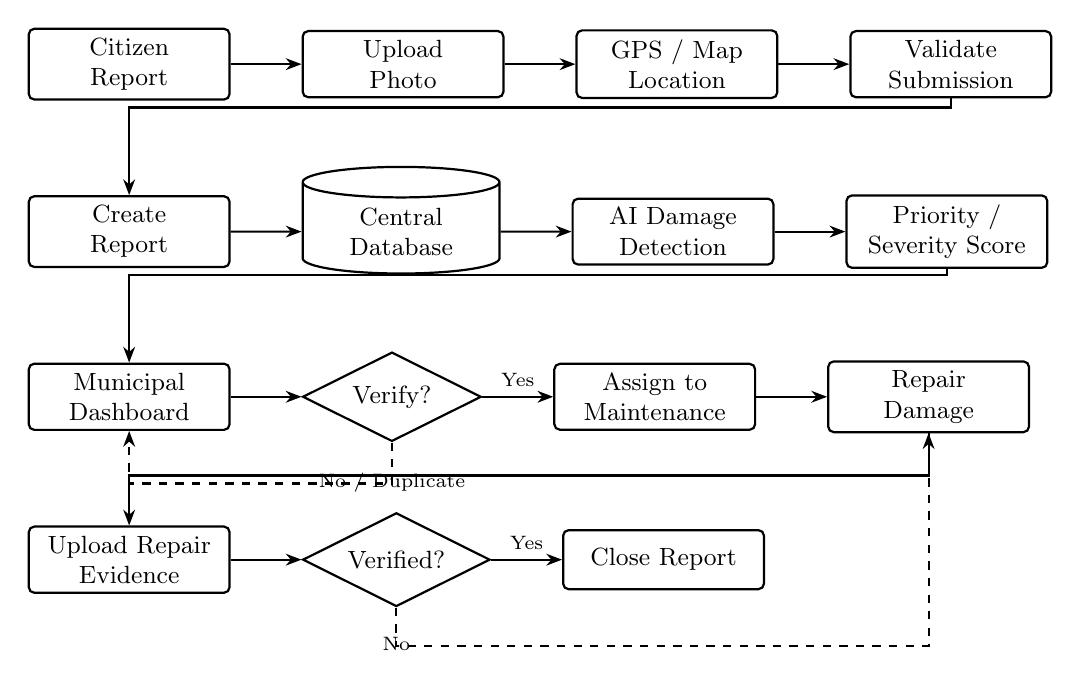
\begin{tikzpicture}[
    node distance=7mm and 9mm,
    box/.style={
        rectangle,
        rounded corners=2pt,
        draw=black,
        thick,
        minimum width=2.55cm,
        minimum height=0.75cm,
        align=center,
        font=\small
    },
    decision/.style={
        diamond,
        draw=black,
        thick,
        minimum width=2.0cm,
        minimum height=0.8cm,
        align=center,
        aspect=2,
        font=\small
    },
    database/.style={
        cylinder,
        draw=black,
        thick,
        shape border rotate=90,
        aspect=0.25,
        minimum width=2.5cm,
        minimum height=0.8cm,
        align=center,
        font=\small
    },
    arrow/.style={
        -{Stealth[length=2mm]},
        thick
    }
]

% ---------------- ROW 1 ----------------

\node[box] (report)
    {Citizen\\Report};

\node[box, right=of report] (photo)
    {Upload\\Photo};

\node[box, right=of photo] (location)
    {GPS / Map\\Location};

\node[box, right=of location] (validate)
    {Validate\\Submission};


\node[box, below=12mm of report] (create)
    {Create\\Report};

\node[database, right=of create] (db)
    {Central\\Database};

\node[box, right=of db] (detect)
    {AI Damage\\Detection};

\node[box, right=of detect] (priority)
    {Priority /\\Severity Score};


\node[box, below=12mm of create] (dashboard)
    {Municipal\\Dashboard};

\node[decision, right=of dashboard] (verify)
    {Verify?};

\node[box, right=of verify] (assign)
    {Assign to\\Maintenance};

\node[box, right=of assign] (repair)
    {Repair\\Damage};


\node[box, below=12mm of dashboard] (evidence)
    {Upload Repair\\Evidence};

\node[decision, right=of evidence] (complete)
    {Verified?};

\node[box, right=of complete] (close)
    {Close Report};


\draw[arrow] (report) -- (photo);
\draw[arrow] (photo) -- (location);
\draw[arrow] (location) -- (validate);

\draw[arrow] (validate) -- ++(0,-0.55)
    -| (create);

\draw[arrow] (create) -- (db);
\draw[arrow] (db) -- (detect);
\draw[arrow] (detect) -- (priority);

\draw[arrow] (priority) -- ++(0,-0.55)
    -| (dashboard);

\draw[arrow] (dashboard) -- (verify);

\draw[arrow] (verify) -- node[above,font=\scriptsize]{Yes} (assign);

\draw[arrow] (assign) -- (repair);

\draw[arrow] (repair) -- ++(0,-1.0)
    -| (evidence);

\draw[arrow] (evidence) -- (complete);

\draw[arrow] (complete) -- node[above,font=\scriptsize]{Yes} (close);

\draw[arrow,dashed]
    (verify)
    -- node[below,font=\scriptsize]{No / Duplicate}
    ++(0,-1.1)
    -| (dashboard);

\draw[arrow,dashed]
    (complete)
    -- node[below,font=\scriptsize]{No}
    ++(0,-1.1)
    -| (repair);

\end{tikzpicture}

\caption{Complete CivicSight workflow from citizen reporting to verified road repair.}
\label{fig:civicsight-workflow}

\end{figure}

\subsection{Practical implementation}

The project will be designed as a responsive web application. Location will be captured through the browser's geolocation facility when permission is given, with map-based selection available as a fallback.

The computer-vision component will use a labelled road-damage dataset and a pre-trained object-detection model that is fine-tuned for the selected damage categories. The aim is not to develop a completely new AI algorithm, but to integrate an existing computer-vision approach into a useful software system.

For the educational prototype, open-source and freely available tools will be preferred so that core functionality does not depend on paid services.


\section{Solution Approach}

CivicSight is primarily a software engineering system in which computer vision is one component. The project will focus on connecting users, reports, locations, automated assessment, business rules, databases, and maintenance workflows reliably.

\subsection{Road-damage assessment}

The image-analysis component will be trained/fine-tuned using a labelled road-damage dataset. The initial system will focus on major road-surface defects such as potholes and pavement cracks.

The model will provide decision-support information rather than making the final maintenance decision. Municipal users will be able to verify or reject automated results.

\subsection{Priority and business rules}

A priority engine will convert assessment information into an actionable priority level. The score may consider:

\begin{itemize}[leftmargin=0.6cm]

    \item type and severity of detected damage,
    \item presence of multiple damage types,
    \item confidence of the automated assessment,
    \item importance of the reported location where relevant,
    \item previous unresolved reports from the same location.

\end{itemize}

The rules will be documented and tested so that the prioritization remains understandable rather than being a hidden decision.

\subsection{System architecture}

The system will follow a three-tier architecture:

\begin{itemize}[leftmargin=0.6cm]

    \item \textbf{Frontend:} interfaces for citizens, municipal personnel, and maintenance teams.

    \item \textbf{Backend:} authentication, report creation, image-analysis requests, location handling, priority calculation, assignment, and status management.

    \item \textbf{Database and storage:} structured records for users, reports, locations, assessments, assignments, repairs, notifications, and status history. Images will be stored separately and referenced by the application.

\end{itemize}

This separation will make the system easier to test, maintain, and extend.

\subsection{Testing and quality assurance}

Testing will cover both individual components and complete workflows. Planned testing includes:

\begin{itemize}[leftmargin=0.6cm]

    \item unit testing of validation and priority logic,
    \item API and integration testing,
    \item database consistency testing,
    \item role and authorization testing,
    \item report lifecycle testing,
    \item image-upload and location validation,
    \item evaluation of computer-vision performance using standard detection metrics.

\end{itemize}

\section{Evaluation Criterion}

The project will be evaluated using measurable system and model outcomes.

\subsection{Primary metrics}

\textbf{Report processing success rate:} percentage of valid submissions that successfully pass through image upload, location capture, report creation, and database storage.

\begin{itemize}[leftmargin=0.6cm]
    \item Target: at least 95\% successful processing for valid test submissions.
    \item Measurement: application logs and database records.
\end{itemize}

\textbf{Road-damage detection performance:} precision, recall, and mean Average Precision (mAP) on a held-out test set.

\subsection{Secondary metrics}

\begin{itemize}[leftmargin=0.6cm]

    \item \textbf{Workflow correctness:} percentage of test cases following valid report transitions.

    \item \textbf{Priority consistency:} percentage of predefined scenarios receiving the expected priority.

    \item \textbf{Response time:} time required for common operations such as report creation and dashboard retrieval.

    \item \textbf{Traceability:} ability to retrieve the complete history of a report, including assignment and repair evidence.

    \item \textbf{Usability:} feedback on the clarity and simplicity of the reporting and administrative interfaces.

\end{itemize}

\subsection{Validation plan}

The team will test the system using controlled reporting scenarios, simulated municipal users, and a separate set of images for model evaluation. Expected and actual system behaviour will be compared across predefined test cases, with failures recorded and addressed during later iterations.

\section{Scalability}

Although the project is designed as a student prototype, its architecture will allow future expansion.

\begin{enumerate}[leftmargin=0.6cm]

    \item \textbf{Scalable in design:} The frontend, backend, database, and model-serving responsibilities will be separated. Database indexing, pagination, and asynchronous image processing can support larger numbers of reports.

    \item \textbf{Extensible in functionality:} Future versions could support additional road-damage categories, mobile applications, vehicle/dashcam reporting, historical road-condition analysis, and integration with municipal systems.

\end{enumerate}

\section{Engine availability heuristic}

The core system can be developed using open-source and freely available technologies. The project will avoid making paid third-party services a requirement.

The main development components include:

\begin{itemize}[leftmargin=0.6cm]

    \item web and REST API development tools,
    \item a relational database,
    \item browser-based geolocation and map visualization,
    \item open-source computer-vision libraries and models,
    \item local or free storage during development,
    \item authentication and role-based access control,
    \item automated testing and source-control tools.

\end{itemize}

Where a cloud service is unnecessary, local development will be preferred. This keeps the educational implementation practical without introducing avoidable costs.

\section{Project scope and deliverables}

\subsection{Initial deliverable}

\begin{itemize}[leftmargin=0.6cm]

    \item Citizen registration/login and road-damage reporting.
    \item Image upload and location capture.
    \item Unique report creation and database storage.
    \item Basic municipal dashboard.
    \item Initial report lifecycle from submission to verification and assignment.
    \item Testing of report creation, validation, authorization, and status transitions.

\end{itemize}

\subsection{Subsequent deliverables}

\begin{itemize}[leftmargin=0.6cm]

    \item Fine-tuned road-damage detection model and backend integration.
    \item Automated damage classification and confidence recording.
    \item Severity and priority scoring.
    \item Map-based dashboard with useful filters.
    \item Maintenance-team assignment and repair tracking.
    \item Before/after repair evidence and final verification.
    \item Analytics and administrative reports.
    \item Final testing, evaluation, and deployment-ready documentation.

\end{itemize}

\section{Risks and mitigations}

\begin{itemize}[leftmargin=0.6cm]

    \item \textbf{Model accuracy:} Road images vary considerably. The model will be evaluated on held-out data, while final decisions remain with authorized users.

    \item \textbf{Location availability:} Users may deny GPS access. Map-based location selection will therefore be provided as an alternative.

    \item \textbf{Duplicate reports:} Similar reports can be flagged using location and time information and reviewed by administrators.

    \item \textbf{Privacy:} Only information needed for reporting and workflow management will be collected, with role-based access to sensitive information.

    \item \textbf{Scope expansion:} Advanced features will remain optional so that the core reporting-to-resolution workflow is completed first.

    \item \textbf{Computing limitations:} Transfer learning and an appropriately sized model will be used to keep training feasible on available student hardware.

    \item \textbf{External dependencies:} Paid APIs will not be required for core functionality; open-source or local alternatives will be preferred.

\end{itemize}

\section{Summary}

CivicSight is an end-to-end platform for managing road-surface damage from the moment a citizen reports it to the point where the repair is verified and closed. It combines geographic reporting, computer-vision-assisted assessment, priority calculation, centralized records, municipal assignment, and repair tracking.

The project is particularly suitable for Software Engineering because its main challenge is not simply training a machine-learning model. The team must design a reliable multi-user system with clear requirements, database relationships, APIs, authentication, business rules, workflows, testing, and traceability. The AI component adds an intelligent layer to a practical public-infrastructure problem while the overall system demonstrates the complete software engineering process.

\end{document}